\documentclass{article}
\usepackage[spanish]{babel}
\usepackage[a4paper,top=2cm,bottom=2cm,left=3cm,right=3cm,marginparwidth=1.75cm]{geometry}
\usepackage[colorlinks=true, allcolors=blue]{hyperref}
\usepackage{tabularx} % para autoajustar las tablas según contenido del texto
\usepackage{changepage} % para ajuste de márgenes
\usepackage{graphicx}

\title{\textbf{Numerología. Ciencia cierta o Superstición.}}
\author{Camilo Riquelme Horta}
\date{25.03.2024}

\begin{document}
	
	\begin{minipage}{0.5\textwidth}
		\begin{flushleft}
			Universidad Mayor \\Facultad de Ciencias, Ingeniería y Tecnología \\Carrera de Data Science
		\end{flushleft}
	\end{minipage}
	\begin{minipage}{0.5\textwidth}
		\begin{flushright}
			Taller de Ciencia de Datos I \\Profesor: Felipe Urbina
		\end{flushright}
	\end{minipage}\\
	
	\begin{minipage}{395px}
		\maketitle
	\end{minipage}
	
	\begin{abstract}
		El texto a continuación entregará una breve información sobre la numerología. Explicando sus pros y contras. Así como una pequeña introducción del como nace esta pseudociencia.
		\\\\Palabras clave: Numerología - Pseudociencia - Ciencia - Superstición.
	\end{abstract}
	
	\section*{Introducción}
	
	La numerología tiene sus orígenes entre los siglos VI al V a.C., con el conocido filósofo griego Pitágoras \cite{wikipedia}. A grandes rasgos, la numerología es una práctica/estudio que busca establecer una relación entre los números y seres vivos a través de “vibración numérica”, indicando que estos podrían estar ligados a fuerzas físicas y/o espirituales promoviendo el entendimiento sobre la forma de actuar de las personas e incluso predecir su futuro, como dice la siguiente cita:\\
	
	\begin{adjustwidth}{1cm}{1cm}
		\small
		\begin{quote}
			“se dice que los números son uno de los conceptos humanos más perfectos y elevados. Según sus practicantes, la numerología es la disciplina que busca investigar la «vibración secreta» de ese código y enseñan a utilizar los números en su beneficio, por medio del estudio de su influencia sobre personas y animales.”\cite{wikipedia}\\
		\end{quote}
	\end{adjustwidth}
	
	Lo anterior deja planteado y nos invita a reflexionar que los números son más que una manera simple de cuantificar lo existente. De cierta forma, la vida se basa en ellos y es esta vibración la que nos guiaría -o nos podría guiar- a lo largo de nuestra existencia. Esta práctica nos insta a considerar la vibración secreta como una realidad, creer en ella e idealizar la idea de un mundo completamente conectado a través de los números.
	
	\section*{Desarrollo: Pros y Contras}
	
	En numerología cada número del 1 al 9 posee un significado y simboliza atributos o características. Se plantea que al analizar ya sea una fecha de nacimiento, nombre, etc. podríamos descubrir ciertas cosas (como la personalidad) de una persona, aunque se plantea que esta práctica podría representar no sólo características humanas, sino también animales. La idea es sumar los números que componen lo que se analizará, la fecha de nacimiento sería el día, más el número del mes, más el año; en el caso de un nombre se contabiliza la posición de la letra en el abecedario, como muestra el Cuadro \ref{tab1}: $(a, j, s)=1; (b, k, t)=2; (c, l, u)=3...$, etc.\cite{ochoa}\\
	
	\begin{table}[htbp] % argumento de posición
		\centering
		\begin{tabular}{|c|c|c|c|c|c|c|c|c|c|c|c|c|c|}
			\hline
			Letra & A & B & C & D & E & F & G & H & I & J & K & L & M \\\hline
			Valor & 1 & 2 & 3 & 4 & 5 & 6 & 7 & 8 & 9 & 1 & 2 & 3 & 4 \\\hline\hline
			Letra & N/Ñ & O & P & Q & R & S & T & U & V & W & X & Y & Z \\\hline
			Valor & 5 & 6 & 7 & 8 & 9 & 1 & 2 & 3 & 4 & 5 & 6 & 7 & 8 \\\hline
		\end{tabular}
		\caption{\label{tab1} Valores numéricos de cada letra en numerología. (Fuente \cite{ochoa})}
	\end{table}
	
	En el caso de que el número resultante de la suma se componga de dos o más dígitos debemos sumar cada dígito hasta que la suma obtenida sea un numero entre 1 y 9 (ejemplo: tenemos el número 124, debemos sumar $1+2+4=7$). Una vez obtenido el número, podremos revisar las interpretaciones correspondientes a él desde los distintos foros/sitios web sobre numerología.\\
	
	\begin{table}[htbp] % argumento de posición
		\centering
		\begin{tabularx}{\textwidth}{|c|X|} % tabularx para autoajustar las tablas según contenido del texto
			\hline
			Número & Significado\\
			\hline
			1 & Representa una personalidad decidida, fuerte, dinámica, valiente, entusiasta e individualista. \\\hline
			2 & La persona que tiene este número es paciente, versátil, servicial, ingeniosa, amable y adaptable. \\\hline
			3 & La personalidad es exuberante, optimista, entusiasta, orgullosa, autoritaria y creativa. \\\hline
			4 & Representa una personalidad metódica, concreta, perseverante, ligada a los valores tradicionales, reflexiva y con muchos talentos. \\\hline
			5 & Quien tiene este número es entusiasta, jovial, intuitivo, independiente, adaptable y dinámico. \\\hline
			6 & Representa una personalidad madura, disponible para las necesidades de los demás, creativa, sensible, comprensiva, sentimental y tenaz. \\\hline
			7 & La persona que tiene este número personal es intuitiva, sensible, emocional, busca la perfección y está dotada de imaginación y creatividad. \\\hline
			8 & La personalidad es ambiciosa y autoritaria, tenaz, orgullosa, magnética, enérgica y obstinada. \\\hline
			9 & Sensibilidad, generosidad, equilibrio, diplomacia, atención, claridad, sentido del deber y amor por los demás son las características positivas de quienes tienen este número personal. \\\hline
		\end{tabularx}
		\caption{\label{tab2} Significado de cada número. (Fuente \cite{ochoa})}
	\end{table}
	
	Realizando ejemplos más concretos (con mi nombre y fecha de nacimiento), veamos qué dice la numerología sobre mí.\\\\
	Mi nombre es  Camilo Nicolás Riquelme Horta. La numerología nos dice que existen dos valores para el nombre, el número del alma (suma de vocales) y el número de la personalidad (suma de consonantes)\cite{clarin}, entonces, ejemplificamos siguiendo el Cuadro \ref{tab1}:
	
	\subsubsection*{Número del alma}
	$3A(1)+3I(9)+3O(6)+2E(5)+1U(3)=61$.\\\\
	Al ser un número de dos dígitos sumo sus componentes, obteniendo: $6+1=7$.\\\\
	Acorde al Cuadro \ref{tab2}: “La persona que tiene este número personal (7) es intuitiva, sensible, emocional, busca la perfección y está dotada de imaginación y creatividad.”
	
	\subsubsection*{Número de la personalidad}
	$3L(3)+2R(9)+2M(4)+2C(3)+1N(5)+1S(1)+1Q(8)+1H(8)+1T(2)=65=11=2$\\\\
	Tenemos que: “La persona que tiene este número (2) es paciente, versátil, servicial, ingeniosa, amable y adaptable.”
	
	\subsubsection*{Fecha de nacimiento}
	Nací el 1 de julio del 2001, entonces:\\\\
	$0+1+0+7+2+0+0+1=11=2$.\\\\
	Obteniendo el mismo resultado y significado que en el número de la personalidad.\\\\
	Una vez realizado lo anterior, observo que mis números son 7, 2 (por mi nombre) y 2 (por mi fecha de nacimiento), por lo que las cualidades anteriormente mencionadas serían aquellas que me representarían. En este caso, apareció en dos ocasiones el número 2, significando que posiblemente estos serían mis atributos principales.
	
	\subsubsection*{Otros ejemplos. Gráficos estadísticos}
	
	A continuación se presentan dos gráficos. Ambos realizan un conteo de los números del 1 al 9 obtenidos tras el proceso enseñado anteriormente con las fechas correspondientes. La Figura \ref{fig:plot} representa la frecuencia anual obtenida por las fechas correspondientes al año 2024. Mientras que, la Figura \ref{fig:plot1} muestra la frecuencia obtenida de algunos estudiantes del curso (incluyéndome).
	
	\begin{figure}[htbp]
		\begin{center}
			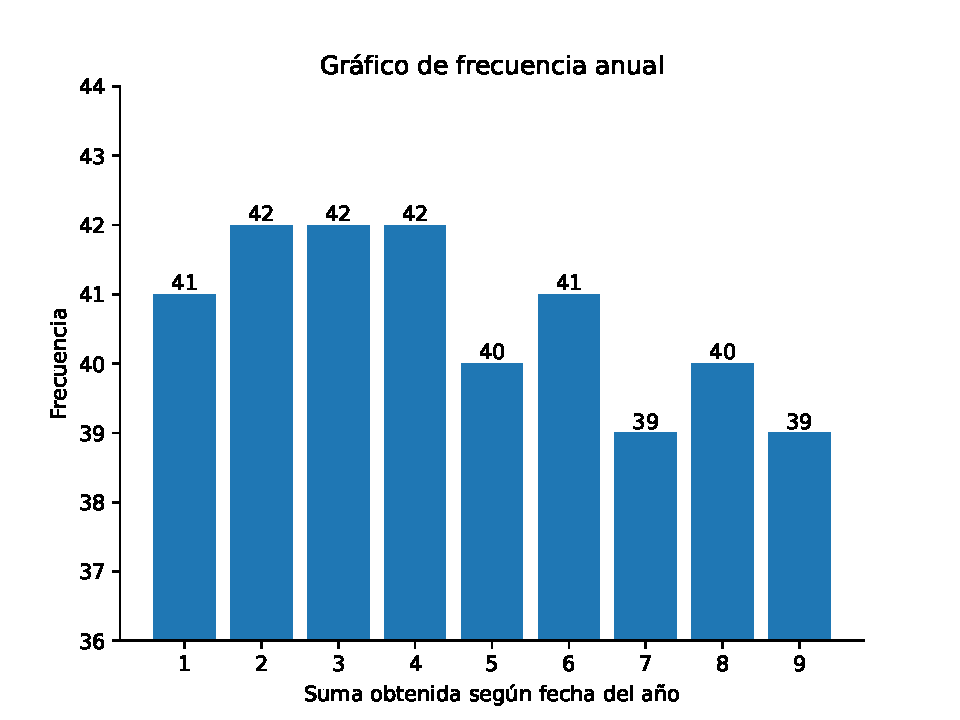
\includegraphics[width = 0.78\textwidth]{figs/anual.pdf}
			\caption{\label{fig:plot} Estadística numerológica 2024.}
		\end{center}
		\begin{center}
			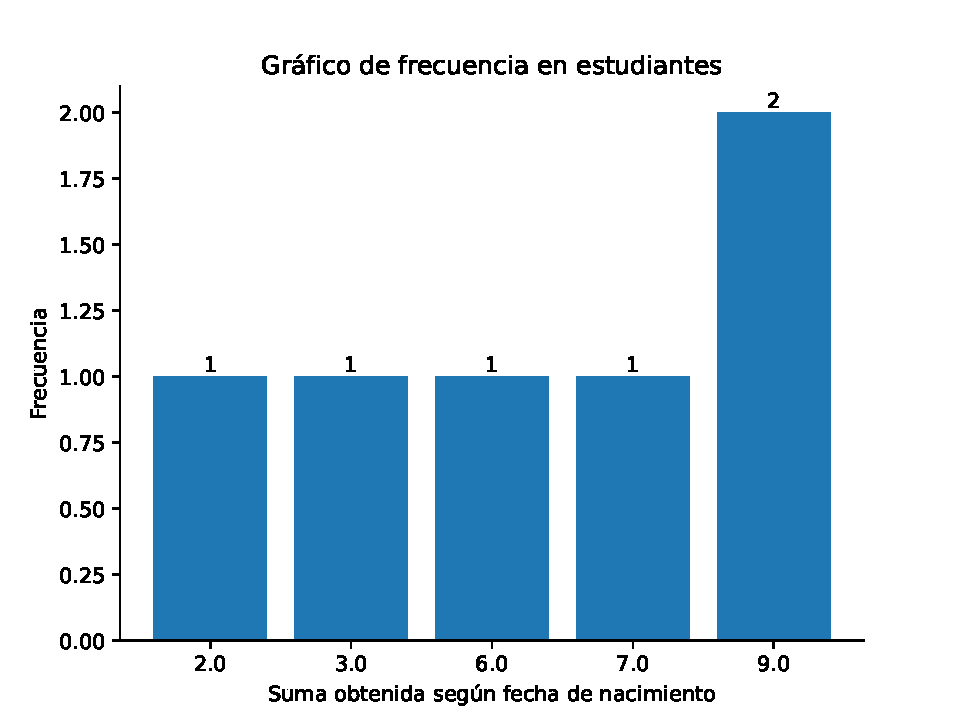
\includegraphics[width = 0.78\textwidth]{figs/taller.pdf}
			\caption{\label{fig:plot1} Estadística de estudiantes.}
		\end{center}
	\end{figure}
	
	Considero que ambos gráficos nos presentan un contenido interesante. Por un lado, en la Figura \ref{fig:plot} podemos observar que quienes nacieron/nacerán este año presentan una distribución bastante uniforme en cuanto a la suma obtenida de sus fechas de nacimiento (esto considerando como si los nacimientos se distribuyesen equitativamente a lo largo del año), esto nos deja con los números 2, 3 y 4 como los más frecuentes, repitiéndose 42 veces cada uno,  mientras que los números 7 y 9 son los menos comunes, registrándose en 39 ocasiones cada uno. Como podemos ver, lo anterior invita a deducir que los nacidos en 2024, tendrían mayor tendencia a generar personalidades basadas en los números 2, 3 y 4 (que podemos revisar en el Cuadro \ref{tab2}). No obstante, la variación no es enorme, considerando que los de mayor frecuencia se diferencian de aquellos con menos frecuentes por tan solo 3 repeticiones.\\\\
	Por otro lado, en la Figura \ref{fig:plot1} logramos captar que existe una pequeña tendencia hacia el número 9 dentro de los 6 (de 10) estudiantes del curso “Taller de Ciencia de Datos I”, propiciando a que si me acerco a uno de ellos tenga más posibilidades de interactuar con una persona de naturaleza asociada a este dígito (revisable desde el Cuadro \ref{tab2}). Además, es posible que dentro de la sala predomine un poco más la personalidad asociada a dicho número o que incluso existan discrepancias por el diferente carácter de cada estudiante.
	
	\subsection*{Pros}
	
	Sirve como una herramienta de orientación, permitiendo la reflexión y el autoconocimiento a través de los números de nuestra vida, ya que comprendiendo sus vibraciones y significados podemos decidir y comprender nuestro actuar, otorgarnos una nueva perspectiva sobre nuestra vida y permitirnos analizar aspectos que tal vez no hayamos considerado antes. La numerología estaría, en tal caso, permitiéndonos tomar decisiones más informadas gracias al hecho de haber ampliado el conocimiento y visión sobre uno mismo “porque nuestra consciencia sabe qué recursos necesitará para gestionar la propia evolución”.\cite{rutenberg}
	
	\subsection*{Contras}
	
	A pesar de presentarse como una muy buena opción para al autoconocimiento y ampliación de la visión en si mismo, la numerología carece de una importante falta de evidencia científica, ya que no existe evidencia empírica que respalde dichas afirmnaciones, prestándose a las distintas creencias de cada ser que confíe en esta pseudociencia. Además de lo anterior, podremos observar que también queda muy condicionada a las distintas interpretaciones de los números \cite{ochoa}, ya que no cuenta con unas reglas universales a seguir, llevando a inconsistencias y provocando distintas “lecturas” de los mismos números.	Si comparamos con otras pseudociencias que busquen determinar comportamiento y cualidades humanas (como la astrología), la numerología simplifica en mayor medida la vida humana, reduciéndola completamente a la intepretación de par de números como pueden ser el nombre o la fecha de nacimiento.
	
	\section*{Conclusión}
	
	En resumen, considero que la numerología antes que ayudarnos a comprender nuestra vida y entorno a través del significado e interpretación de los números, nos acerca mucho más al autoengaño a través de una supersitición, además de hacernos seguir creencias erróneas debido a la subjetividad existente en la interpretación final. Como punto extra, ya hace años, esta práctica fue relegada por la comunidad científica como una pseudociencia y dejó de ser considerada una disciplina matemática, siendo vista como algo subjetivo y emocional.\cite{wikipedia}\\
	
	\newpage
	
	\begin{thebibliography}{99}
		
		\bibitem{wikipedia}
		Numerología.
		Wikipedia, la enciclopedia libre.
		\url{https://es.wikipedia.org/w/index.php?title=Numerolog%C3%ADa&oldid=154243346}
		[Consulta: 25 de marzo de 2024].
		
		\bibitem{clarin}
		Numerología de tu nombre: cómo calcularlo y qué significa.
		Clarín, 12 de agosto de 2020.
		\url{https://www.clarin.com/astrologia/numerologia-nombre-apellido-significado-numeros_0_Voru3x7nb.html}
		[Consulta: 5 de abril de 2024]
		
		\bibitem{ochoa}
		Ochoa, Andrea.
		Utiliza la numerología para balancear tus días.
		Architectural Digest, 21 de febrero de 2022.
		\url{https://www.admagazine.com/articulos/numerologia-que-es-y-como-utilizarla-en-el-la-vida-diaria}
		[Consulta: 25 de marzo de 2024].
		
		\bibitem{rutenberg}
		Rutenberg, Julieta.
		Cómo saber tu número personal: tu misión de vida, según tu fecha de nacimiento.
		Clarín, 1 de agosto de 2020.
		\url{https://www.clarin.com/astrologia/numerologia-numero-personal-mision-de-vida-nacimiento_0_9n5BfjgHt.html}
		[Consulta: 25 de marzo de 2024].
		
	\end{thebibliography}

\end{document}